\chapterauthor{Bernd Krupinski}
\subsection{Gauge Control Implementierung}

Die Implementierung der Gauge Control erfolgte in der Windows Presentation Foundation (WPF) über eine Custom Control. Zur Darstellung der Skala(1) und dem Zeiger(2) wurden jeweils ein Canvas verwendet. Ein Canvas stellt in WPF eine Zeichenoberfläche dar.\\



Das Control stellt eine Reihe an Variablen zur Verfügung. Diese ermöglichen es dem Entwickler das Control mit Hilfe von wenigen Zeilen Code stark anzupassen. 
\begin{figure}[ht]
	\centering
	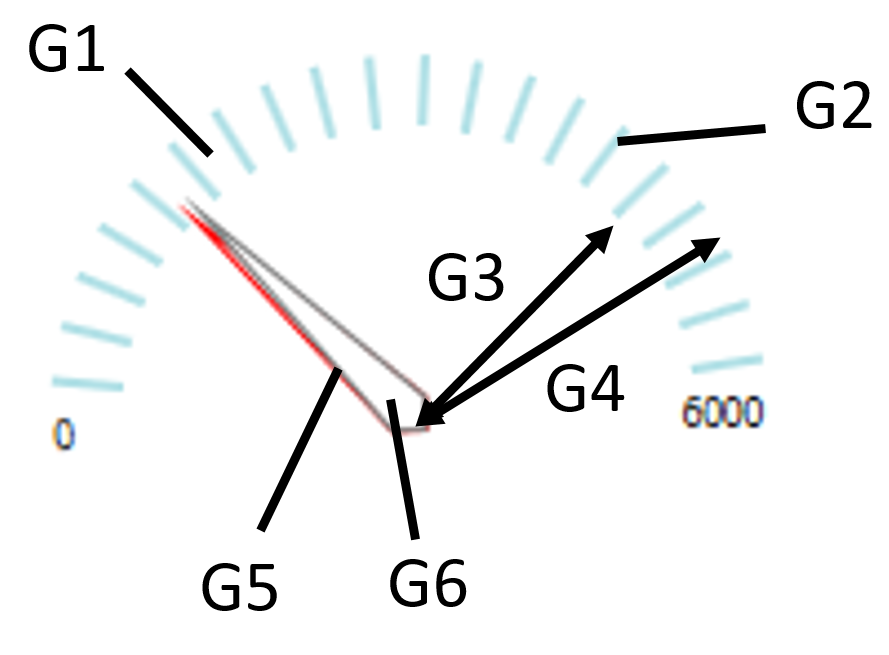
\includegraphics[width=0.6\textwidth]{GaugeDetails}
	\caption{Gauge Control Details}
	\label{fig:gauge}
\end{figure}
Umfassen dabei sind visuelle Parameter wie Kreishintergrundfarbe(G1), Strichlänge, Strichfarbe, Strichanzahl(G2), innerer Radius(G3), Nadellänge, Nadelfarbe(G6) oder Nadelfüllfarbe(G5). Zusätzlich dazu funktionelle Parameter wie Maximalwert, Minimalwert, aktueller Wert etc.\\\\

Das Canvas Control benutzt den Render Zyklus von WPF. Das heißt dass von unserer Seite das Canvas nur geändert werden muss, sollte einer der genannten Variablen sich verändern, also ein neu zeichnen des Tachometers notwendig ist.\\
Dies geschieht in 2 Schritten. \\
\begin{itemize}
	\item Zeichnen des Hintergrunds (Canvas 1)
	\item Zeichnen der Nadel (Canvas 2)
\end{itemize}

Der Hintergrund besteht wiederum aus 2 Teilen. \\

\begin{itemize}
	\item Der kreisförmige Hintergrund.
	\item Halbkreis aus Strichen.
\end{itemize}
Während die Striche mit einer Menge an Strich-Formen entlang des inneren Radius mit der Länge Äußerer Radius(G4) - Innerer Radius, einfach gelöst wird, stellt der Hintergrund eine etwas interessante Problematik.\\
Zwar gibt es eine Ellipsen Form für WPF's Canvas Control, allerdings besteht die Anforderung aus keiner rein einfarbigen Ellipse, sondern stattdessen aus einer zwei geteilte Form wie unten abgebildet.
\begin{figure}[ht]
	\centering
	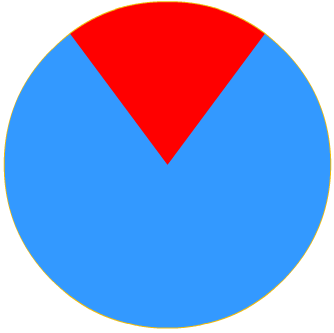
\includegraphics[width=0.6\textwidth]{GaugeForm}
	\caption{Gauge Control Details}
	\label{fig:gauge}
\end{figure}
Stattdessen wird ein Polygon benutzt. Ein Polygon ist eine mit einer Linie verbundene, Menge an Punkten. Optional kann die daraus entstehende Fläche mit einer Farbe gefüllt werden.\\
Um die gewünschte Form zu erzielen, werden 2 Polygone gezeichnet. Das eine (blau) umschließt das andere (rot) und bilden zusammen einen vollen Kreis.\\
\\
Die Nadel wird genau wie der Hintergrund über ein Polygon gezeichnet. Dabei wird die Nadel selbst auf dem Canvas stets richtung Osten gezeichnet. Damit die Nadel schließlich auf den entsprechenden Winkel zeigt, der den aktuellen Wert entspricht, wird nicht die Nadel schräg gezeichnet, sondern stattdessen das Canvas selbst über eine Rotations-Transformation gedreht.
